\tableofcontents

\newpage


\section{Описание метода}
В качестве аппроксимирующей функции используется многочлен первой степени $P_{1}(x)$) = $ax + b$.\\
Введём обозначения:\\
$SX$ = $\sum_{i=1}^{n}x_{i}$, $SXX$ = $\sum_{i=1}^{n}x_{i}^{2}$, $SY$ = $\sum_{i=1}^{n}y_{i}$, $SXY$ = $\sum_{i=1}^{n}x_{i}y_{i}$\\
И вычисляем коэффициенты $a$ и $b$ из системы уравнений:
\begin{equation*}
 \begin{cases}
   aSXX + bSX = SXY,
   \\
   aSX + bn = SY.
 \end{cases}
\end{equation*}
Далее при помощи аппроксимирующего многочлена строим линейную модель.

\section{Блок-схема численного метода}
\begin{figure}[H]
    \centering
    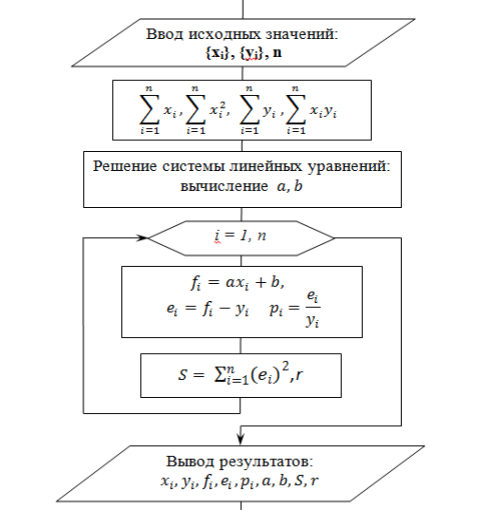
\includegraphics[scale=0.5]{img/block-scheme}
\end{figure}

\section{Listing реализованного численного метода}
\tiny
\begin{verbatim}
    size_t n = x_axis.size();
    double sx = 0;
    double sxx = 0;
    double sy = 0;
    double sxy = 0;
    for (int i = 0; i < n; i++) {
        sx += x_axis.at(i);
        sxx += x_axis.at(i) * x_axis.at(i);
        sy += y_axis.at(i);
        sxy += x_axis.at(i) * y_axis.at(i);
    }
    a = (sxy * n - sx * sy) / (sxx * n - sx * sx);
    b = (sy - sx * a) / n;
    double worst_el = 0;
    size_t iter = 0;
    for (int i = 0; i < x_new.size(); i++) {
        double f = a * x_new[i] + b;
        F.push_back(f);
        double epsilon = std::abs(f - y_axis.at(i));
        double p = epsilon/y_axis.at(i);
        if (p > worst_el) {
            iter = i;
            worst_el = p;
        }
    }
    return iter;
\end{verbatim}
\normalsize


\section{Examples}
исходная функция: $x^2$\par
шум: $\pm$0.5\\
\small
\begin{verbatim}
    std::vector<double> _x = {0, 0.5, 1, 1.5, 2, 2.5, 3, 3.5, 4, 4.5, 5, 5.5, 6, 6.5, 7};
\end{verbatim}
\begin{figure}[h]
    \begin{subfigure}{0.5\textwidth}
        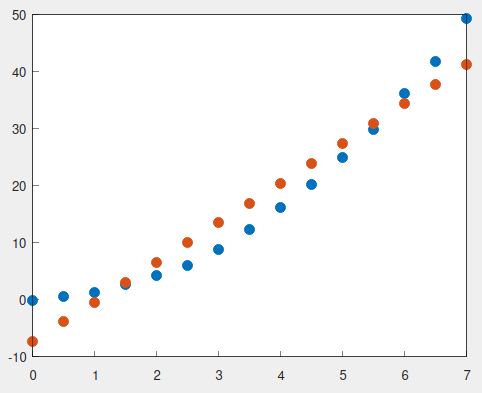
\includegraphics[width=0.9\linewidth, height=6cm]{img/graphic_1}
        \caption{a: 6.94895 , b: -7.37446}
    \end{subfigure}
    \begin{subfigure}{0.5\textwidth}
        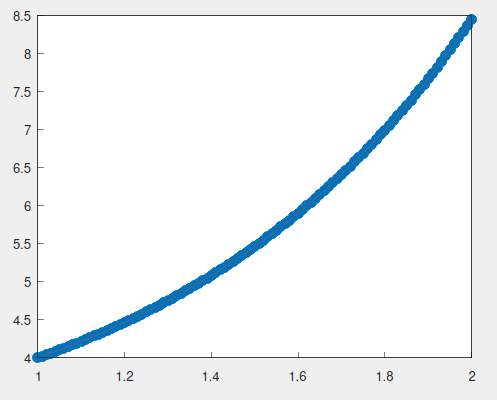
\includegraphics[width=0.9\linewidth, height=6cm]{img/graphic_2}
        \caption{a: 6.94895 , b: -7.37446}
    \end{subfigure}
\end{figure}


\begin{verbatim}
    std::vector<double> _x = {0.1, 0.2, 0.3, 0.4, 0.5, 0.6, 0.7, 0.8, 0.9, 1, 1.1, 1.2, 1.3, 1.4, 1.5};
\end{verbatim}
\begin{figure}[h]
    \begin{subfigure}{0.5\textwidth}
        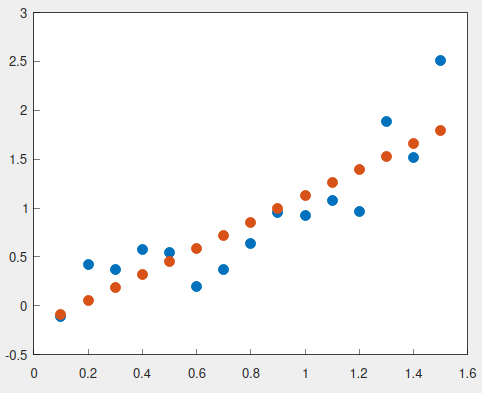
\includegraphics[width=0.9\linewidth, height=6cm]{img/graphic_3}
        \caption{a: 1.34475 , b: -0.218933}
    \end{subfigure}
    \begin{subfigure}{0.5\textwidth}
        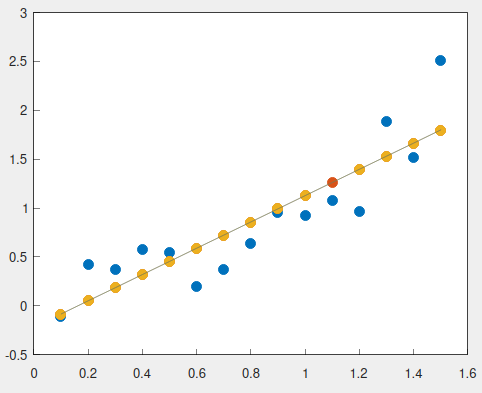
\includegraphics[width=0.9\linewidth, height=6cm]{img/graphic_4}
        \caption{a: 1.34475 , b: -0.218933}
    \end{subfigure}
\end{figure}

\section{Вывод}
Метод наименьших квадратов может быть реализован при помощи нескольких видов функций. Выбор наилучшей аппроксимирующей функции определяется значением
среднеквадратического отклонения. В связи с этим следует:
\begin{enumerate}
    \item по методу наименьших квадратов определить несколько аппроксимирующих функций.
    \item по критерию наименьшего среднеквадратического отклонения выбрать наиболее подходящую функцию.
\end{enumerate}
